%\VignetteIndexEntry{Examples}
%\VignetteEngine{knitr::knitr}
\documentclass[12pt]{article}\usepackage[]{graphicx}\usepackage[]{color}
% maxwidth is the original width if it is less than linewidth
% otherwise use linewidth (to make sure the graphics do not exceed the margin)
\makeatletter
\def\maxwidth{ %
  \ifdim\Gin@nat@width>\linewidth
    \linewidth
  \else
    \Gin@nat@width
  \fi
}
\makeatother

\definecolor{fgcolor}{rgb}{0.345, 0.345, 0.345}
\newcommand{\hlnum}[1]{\textcolor[rgb]{0.686,0.059,0.569}{#1}}%
\newcommand{\hlstr}[1]{\textcolor[rgb]{0.192,0.494,0.8}{#1}}%
\newcommand{\hlcom}[1]{\textcolor[rgb]{0.678,0.584,0.686}{\textit{#1}}}%
\newcommand{\hlopt}[1]{\textcolor[rgb]{0,0,0}{#1}}%
\newcommand{\hlstd}[1]{\textcolor[rgb]{0.345,0.345,0.345}{#1}}%
\newcommand{\hlkwa}[1]{\textcolor[rgb]{0.161,0.373,0.58}{\textbf{#1}}}%
\newcommand{\hlkwb}[1]{\textcolor[rgb]{0.69,0.353,0.396}{#1}}%
\newcommand{\hlkwc}[1]{\textcolor[rgb]{0.333,0.667,0.333}{#1}}%
\newcommand{\hlkwd}[1]{\textcolor[rgb]{0.737,0.353,0.396}{\textbf{#1}}}%
\let\hlipl\hlkwb

\usepackage{framed}
\makeatletter
\newenvironment{kframe}{%
 \def\at@end@of@kframe{}%
 \ifinner\ifhmode%
  \def\at@end@of@kframe{\end{minipage}}%
  \begin{minipage}{\columnwidth}%
 \fi\fi%
 \def\FrameCommand##1{\hskip\@totalleftmargin \hskip-\fboxsep
 \colorbox{shadecolor}{##1}\hskip-\fboxsep
     % There is no \\@totalrightmargin, so:
     \hskip-\linewidth \hskip-\@totalleftmargin \hskip\columnwidth}%
 \MakeFramed {\advance\hsize-\width
   \@totalleftmargin\z@ \linewidth\hsize
   \@setminipage}}%
 {\par\unskip\endMakeFramed%
 \at@end@of@kframe}
\makeatother

\definecolor{shadecolor}{rgb}{.97, .97, .97}
\definecolor{messagecolor}{rgb}{0, 0, 0}
\definecolor{warningcolor}{rgb}{1, 0, 1}
\definecolor{errorcolor}{rgb}{1, 0, 0}
\newenvironment{knitrout}{}{} % an empty environment to be redefined in TeX

\usepackage{alltt}
\usepackage[cm]{fullpage}
\usepackage{hyperref}
\usepackage{amssymb,amsmath}
\DeclareMathOperator*{\minimize}{minimize}
\IfFileExists{upquote.sty}{\usepackage{upquote}}{}
\begin{document}

\title{PeakSegDisk usage examples}
\author{Toby Dylan Hocking}
\maketitle

Welcome to PeakSegDisk, an R package for optimal peak
detection in very large count data sequences. 



\section{Related work}

The PeakSeg R packages contain algorithms for inferring optimal
segmentation models subject to the constraint that up changes must be
followed by down changes, and vice versa. This ensures that the model
can be interpreted in terms of peaks (after up changes) and background
(after down changes). 

\begin{description}
\item[PeakSegDP] the historically first PeakSeg package,
  \url{https://CRAN.R-project.org/package=PeakSegDP} provides a
  heuristic quadratic time algorithm for computing models from 1 to S
  segments for a single sample. This was the original algorithm
  described in our ICML'15 paper,
  \url{http://jmlr.org/proceedings/papers/v37/hocking15.html}, but it
  is neither fast nor optimal, so in practice we recommend to use our
  newer packages below instead.
\item[PeakSegOptimal]
  \url{https://CRAN.R-project.org/package=PeakSegOptimal} provides
  log-linear time algorithms for computing optimal models with
  multiple peaks for a single sample. The algorithms are faster and
  more accurate than PeakSegDP, \url{https://arxiv.org/abs/1703.03352}
\item[PeakSegDisk] \url{https://github.com/tdhock/PeakSegDisk}
  provides an on-disk implementation of optimal log-linear algorithms
  for computing multiple peaks in a single sample. Computes same
  models as PeakSegOptimal but works for much larger data sets because
  disk is used for storage instead of memory.
  \url{https://arxiv.org/abs/1810.00117}
\item[PeakSegJoint] \url{https://CRAN.R-project.org/package=PeakSegJoint}
  provides a fast heuristic algorithm for computing models with a single
  common peak in $0,...,S$
  samples. \url{https://arxiv.org/abs/1506.01286}
\item[PeakSegPipeline]
  \url{https://github.com/tdhock/PeakSegPipeline} provides a pipeline
  for genome-wide peak calling using the other PeakSeg packages. 
\end{description}

The remainder of this vignette is dedicated to an explanation of how
to use PeakSegDisk.

\section{Simulate a noisy integer vector with changes}

The first example we will treat is detecting peaks in a vector of
integer data, with possibly the same values at adjacent
positions. This is an inefficient representation for large genomic
data, but it is the typical output from simulation functions like
\texttt{rpois}:

\begin{knitrout}
\definecolor{shadecolor}{rgb}{0.969, 0.969, 0.969}\color{fgcolor}\begin{kframe}
\begin{alltt}
\hlstd{sim.seg} \hlkwb{<-} \hlkwa{function}\hlstd{(}\hlkwc{seg.mean}\hlstd{,} \hlkwc{size.mean}\hlstd{=}\hlnum{15}\hlstd{)\{}
  \hlstd{seg.size} \hlkwb{<-} \hlkwd{rpois}\hlstd{(}\hlnum{1}\hlstd{, size.mean)}
  \hlkwd{rpois}\hlstd{(seg.size, seg.mean)}
\hlstd{\}}
\hlkwd{set.seed}\hlstd{(}\hlnum{1}\hlstd{)}
\hlstd{seg.mean.vec} \hlkwb{<-} \hlkwd{c}\hlstd{(}\hlnum{1.5}\hlstd{,} \hlnum{3.5}\hlstd{,} \hlnum{0.5}\hlstd{,} \hlnum{4.5}\hlstd{,} \hlnum{2.5}\hlstd{)}
\hlstd{z.list} \hlkwb{<-} \hlkwd{lapply}\hlstd{(seg.mean.vec, sim.seg)}
\hlstd{(z.rep.vec} \hlkwb{<-} \hlkwd{unlist}\hlstd{(z.list))}
\end{alltt}
\begin{verbatim}
#>  [1] 3 0 3 4 2 2 0 0 0 2 1 2 9 3 5 6 2 4 1 2 3 0 3 6 3 3 0 1 1 1 0 1 0 1 1
#> [36] 1 0 0 1 0 0 4 7 4 3 2 2 3 4 5 4 7 3 4 3 5 3 4 4 2 4 2 2 2 5 4 2 4 6 2
#> [71] 3 2 2 3 1
\end{verbatim}
\end{kframe}
\end{knitrout}

From the output above it is clear that these simulated data are
integers, with some identical values at adjacent positions. 

Below we put these data into a data table in order to plot them along
with the model using ggplot2:

\begin{knitrout}
\definecolor{shadecolor}{rgb}{0.969, 0.969, 0.969}\color{fgcolor}\begin{kframe}
\begin{alltt}
\hlstd{count.df} \hlkwb{<-} \hlkwd{data.frame}\hlstd{(}
  \hlkwc{chrom}\hlstd{=}\hlstr{"chrUnknown"}\hlstd{,}
  \hlkwc{chromStart}\hlstd{=}\hlnum{0}\hlopt{:}\hlstd{(}\hlkwd{length}\hlstd{(z.rep.vec)}\hlopt{-}\hlnum{1}\hlstd{),}
  \hlkwc{chromEnd}\hlstd{=}\hlnum{1}\hlopt{:}\hlkwd{length}\hlstd{(z.rep.vec),}
  \hlkwc{count}\hlstd{=z.rep.vec)}
\hlkwd{library}\hlstd{(ggplot2)}
\hlstd{gg.count} \hlkwb{<-} \hlkwd{ggplot}\hlstd{()}\hlopt{+}
  \hlkwd{xlab}\hlstd{(}\hlstr{"position"}\hlstd{)}\hlopt{+}
  \hlkwd{geom_point}\hlstd{(}\hlkwd{aes}\hlstd{(}
    \hlstd{chromEnd, count),}
    \hlkwc{shape}\hlstd{=}\hlnum{1}\hlstd{,}
    \hlkwc{data}\hlstd{=count.df)}
\hlstd{gg.count}
\end{alltt}
\end{kframe}

{\centering 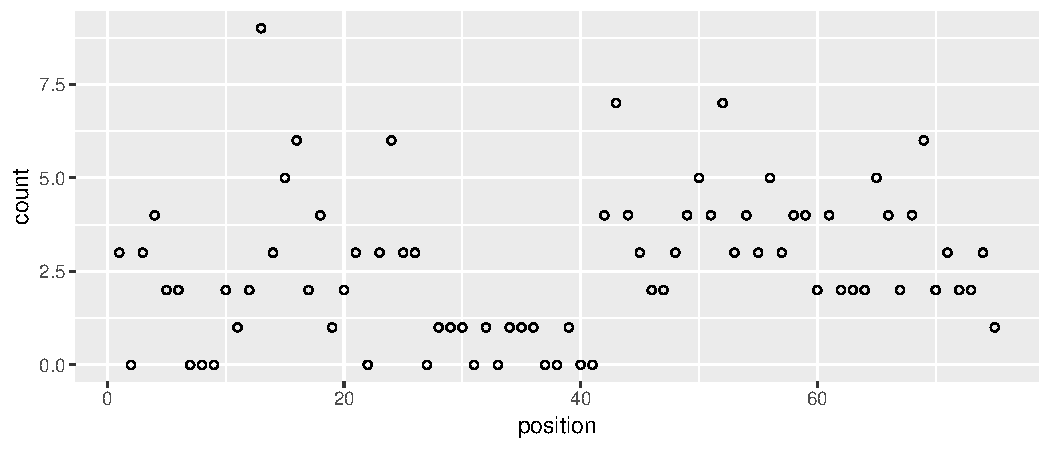
\includegraphics[width=\maxwidth]{figure/ggcount-1} 

}



\end{knitrout}

The true changepoints in the simulation are shown below.

\begin{knitrout}
\definecolor{shadecolor}{rgb}{0.969, 0.969, 0.969}\color{fgcolor}\begin{kframe}
\begin{alltt}
\hlstd{n.segs} \hlkwb{<-} \hlkwd{length}\hlstd{(seg.mean.vec)}
\hlstd{seg.size.vec} \hlkwb{<-} \hlkwd{sapply}\hlstd{(z.list, length)}
\hlstd{seg.end.vec} \hlkwb{<-} \hlkwd{cumsum}\hlstd{(seg.size.vec)}
\hlstd{change.vec} \hlkwb{<-} \hlstd{seg.end.vec[}\hlopt{-}\hlstd{n.segs]}\hlopt{+}\hlnum{0.5}
\hlstd{change.df} \hlkwb{<-} \hlkwd{data.frame}\hlstd{(}
  \hlkwc{changepoint}\hlstd{=change.vec)}
\hlstd{gg.change} \hlkwb{<-} \hlstd{gg.count}\hlopt{+}
  \hlkwd{geom_vline}\hlstd{(}\hlkwd{aes}\hlstd{(}
    \hlkwc{xintercept}\hlstd{=changepoint,} \hlkwc{color}\hlstd{=model),}
    \hlkwc{data}\hlstd{=}\hlkwd{data.frame}\hlstd{(change.df,} \hlkwc{model}\hlstd{=}\hlstr{"simulation"}\hlstd{))}\hlopt{+}
  \hlkwd{scale_color_manual}\hlstd{(}
    \hlkwc{values}\hlstd{=}\hlkwd{c}\hlstd{(}
      \hlkwc{simulation}\hlstd{=}\hlstr{"black"}\hlstd{,}
      \hlkwc{fitted}\hlstd{=}\hlstr{"green"}\hlstd{))}
\hlstd{gg.change}
\end{alltt}
\end{kframe}

{\centering 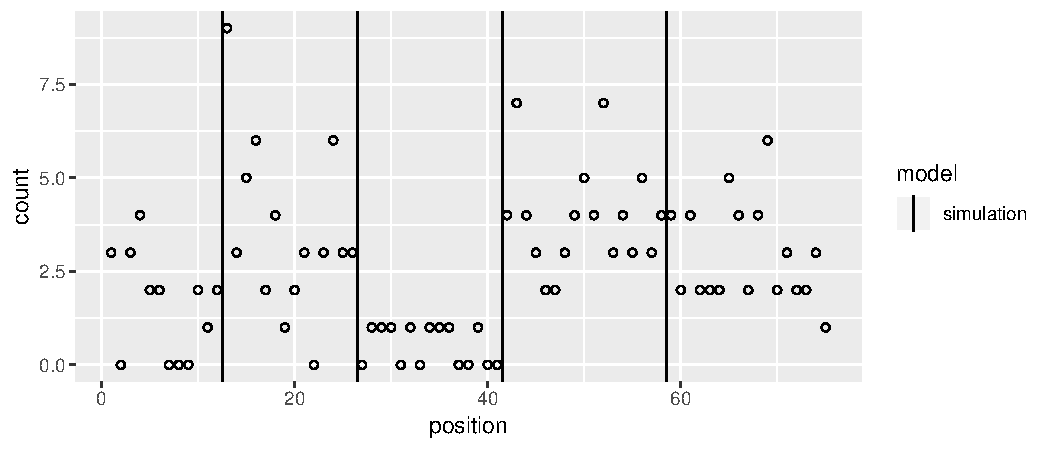
\includegraphics[width=\maxwidth]{figure/unnamed-chunk-2-1} 

}



\end{knitrout}

\section{Segment a vector of integers}

Let $z_1, \dots, z_n\in\mathbb Z_+$ be the sequence of $n$
non-negative count data in z.rep.vec, and let $w_1=\cdots=w_n=1$ be
weights which are all 1. The peak detection algorithm computes the
solution to the following optimization problem:

\begin{align*}
  \minimize_{
    \substack{
    \mathbf m\in\mathbb R^n,\ \mathbf s\in\{0, 1\}^n\\
\mathbf c\in\{-1, 0,1\}^{n-1}\\
}
    } &\ \ 
  \sum_{i=1}^n w_i \ell(m_i, z_i) + \lambda \sum_{i=1}^{n-1} I(c_i = 1) \\
  \text{subject to\ \ } &\ \text{no change: }c_i = 0 \Rightarrow m_i = m_{i+1}\text{ and }s_i=s_{i+1}
  \nonumber\\
&\ \text{go up: }c_i = 1 \Rightarrow m_i \leq m_{i+1}\text{ and }(s_i,s_{i+1})=(0,1),
  \nonumber\\
&\ \text{go down: } c_i = -1 \Rightarrow m_i \geq m_{i+1}\text{ and }(s_i,s_{i+1})=(1,0),\\
  & \ \text{start and end down: } s_1=s_n=0.\nonumber
\end{align*}
where $\ell(m, z)= m - z\log m$ is the Poisson loss. The optimization
variables are $m_i$ for the segment mean, $s_i$ for hidden state, and
$c_i$ for type of changepoint. The penalty term is proportional to the number of
changepoint variables $c_i$ which are equal to 1 (which is the same as
the number of peaks in the resulting model).

To run the peak detection algorithm a numeric penalty parameter
$\lambda\geq 0$ must be specified by the user. The smallest value is 0
which yields max peaks, and the largest value is Inf which yields no
peaks.  The code below runs the peak detection algorithm on this count
data vector, using the penalty parameter $\lambda = 10.5$:

\begin{knitrout}
\definecolor{shadecolor}{rgb}{0.969, 0.969, 0.969}\color{fgcolor}\begin{kframe}
\begin{alltt}
\hlstd{fit} \hlkwb{<-} \hlkwd{list}\hlstd{()}
\hlstd{(fit}\hlopt{$}\hlstd{vec} \hlkwb{<-} \hlstd{PeakSegDisk}\hlopt{::}\hlkwd{PeakSegFPOP_vec}\hlstd{(z.rep.vec,} \hlnum{10.5}\hlstd{))}
\end{alltt}
\begin{verbatim}
#> $segments
#>         chrom chromStart chromEnd     status     mean
#> 1: chrUnknown         69       75 background 2.166670
#> 2: chrUnknown         41       69       peak 3.714290
#> 3: chrUnknown         26       41 background 0.533333
#> 4: chrUnknown         12       26       peak 3.571430
#> 5: chrUnknown          0       12 background 1.583330
#> 
#> $loss
#>    penalty segments peaks bases bedGraph.lines mean.pen.cost total.loss
#> 1:    10.5        5     2    75             60    0.01507491  -19.86938
#>    equality.constraints mean.intervals max.intervals  megabytes seconds
#> 1:                    0            4.6             8 0.02745438   0.011
#> 
#> $data
#>          chrom chromStart chromEnd count
#>  1: chrUnknown          0        1     3
#>  2: chrUnknown          1        2     0
#>  3: chrUnknown          2        3     3
#>  4: chrUnknown          3        4     4
#>  5: chrUnknown          4        6     2
#>  6: chrUnknown          6        9     0
#>  7: chrUnknown          9       10     2
#>  8: chrUnknown         10       11     1
#>  9: chrUnknown         11       12     2
#> 10: chrUnknown         12       13     9
#> 11: chrUnknown         13       14     3
#> 12: chrUnknown         14       15     5
#> 13: chrUnknown         15       16     6
#> 14: chrUnknown         16       17     2
#> 15: chrUnknown         17       18     4
#> 16: chrUnknown         18       19     1
#> 17: chrUnknown         19       20     2
#> 18: chrUnknown         20       21     3
#> 19: chrUnknown         21       22     0
#> 20: chrUnknown         22       23     3
#> 21: chrUnknown         23       24     6
#> 22: chrUnknown         24       26     3
#> 23: chrUnknown         26       27     0
#> 24: chrUnknown         27       30     1
#> 25: chrUnknown         30       31     0
#> 26: chrUnknown         31       32     1
#> 27: chrUnknown         32       33     0
#> 28: chrUnknown         33       36     1
#> 29: chrUnknown         36       38     0
#> 30: chrUnknown         38       39     1
#> 31: chrUnknown         39       41     0
#> 32: chrUnknown         41       42     4
#> 33: chrUnknown         42       43     7
#> 34: chrUnknown         43       44     4
#> 35: chrUnknown         44       45     3
#> 36: chrUnknown         45       47     2
#> 37: chrUnknown         47       48     3
#> 38: chrUnknown         48       49     4
#> 39: chrUnknown         49       50     5
#> 40: chrUnknown         50       51     4
#> 41: chrUnknown         51       52     7
#> 42: chrUnknown         52       53     3
#> 43: chrUnknown         53       54     4
#> 44: chrUnknown         54       55     3
#> 45: chrUnknown         55       56     5
#> 46: chrUnknown         56       57     3
#> 47: chrUnknown         57       59     4
#> 48: chrUnknown         59       60     2
#> 49: chrUnknown         60       61     4
#> 50: chrUnknown         61       64     2
#> 51: chrUnknown         64       65     5
#> 52: chrUnknown         65       66     4
#> 53: chrUnknown         66       67     2
#> 54: chrUnknown         67       68     4
#> 55: chrUnknown         68       69     6
#> 56: chrUnknown         69       70     2
#> 57: chrUnknown         70       71     3
#> 58: chrUnknown         71       73     2
#> 59: chrUnknown         73       74     3
#> 60: chrUnknown         74       75     1
#>          chrom chromStart chromEnd count
#> 
#> attr(,"class")
#> [1] "PeakSegFPOP_df"  "PeakSegFPOP_dir" "list"
\end{verbatim}
\end{kframe}
\end{knitrout}


The model output list above includes \verb|segments|, a data table with
one row for each segment mean, and \verb|loss|, a data table with one
row that reports the model meta-data. Of interest are:

\begin{itemize}
\item \verb|penalty|, the user-provided penalty value,
\item \verb|segments|, the number of segments,
\item \verb|peaks|, the number of peaks (even-numbered segments),
\item \verb|bases|, the number of data points in repetitive form (not run-length encoding),
\item \verb|bedGraph.lines|, the number of data points in run-length encoding form,
\item \verb|mean.pen.cost|, the optimal mean loss plus penalty*peaks,
\item \verb|total.loss|, the optimal total Poisson loss over all data points, 
\item \verb|equality.constraints|, the number of adjacent segment
  means that are equal in the optimal solution. Note that when this
  number is greater than 0, then there are some active equality
  constraints, and the optimal model is therefore not feasible for the
  strict inequality constraints, which implies that the optimum of the
  problem with strict inequality constraints is undefined, i.e. for
  any sub-optimal solution that satisfies the strict inequality
  constraints, we can find a lower cost solution that satifies the
  strict inequality constraints (but is still sub-optimal), by getting
  closer to the solution with active equality constraints.
\item \verb|megabytes|, the storage space on disk used by the solver,
\item \verb|seconds|, the amount of time used by the solver,
\item \verb|mean.intervals|, \verb|max.intervals|, statistics over all intervals
  (candidate changepoints) computed by the functional pruning
  algorithm, useful for analyzing computational complexity, which is
  linear in the number of intervals.
\end{itemize}
Note in particular that \verb|PeakSegFPOP_vec| internally uses \verb|rle| to
construct a run-length encoding, which is passed to the solver to save
time/storage. In this case the repetitive integer data vector contains
75 elements but the coverage.bedGraph data file
contains only 60 lines. In real genomic data
sets the difference is typically much larger.

\begin{knitrout}
\definecolor{shadecolor}{rgb}{0.969, 0.969, 0.969}\color{fgcolor}\begin{kframe}
\begin{alltt}
\hlstd{gg.change}\hlopt{+}
  \hlkwd{geom_segment}\hlstd{(}\hlkwd{aes}\hlstd{(}
    \hlstd{chromStart}\hlopt{+}\hlnum{0.5}\hlstd{, mean,} \hlkwc{xend}\hlstd{=chromEnd}\hlopt{+}\hlnum{0.5}\hlstd{,} \hlkwc{yend}\hlstd{=mean,} \hlkwc{color}\hlstd{=model),}
    \hlkwc{data}\hlstd{=}\hlkwd{data.frame}\hlstd{(fit}\hlopt{$}\hlstd{vec}\hlopt{$}\hlstd{segments,} \hlkwc{model}\hlstd{=}\hlstr{"fitted"}\hlstd{))}
\end{alltt}
\end{kframe}

{\centering 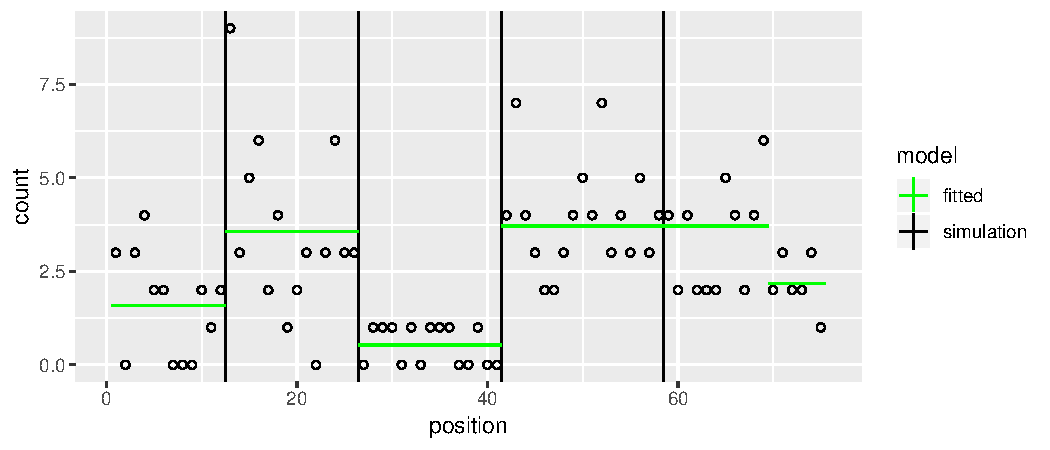
\includegraphics[width=\maxwidth]{figure/unnamed-chunk-4-1} 

}



\end{knitrout}

It is clear from the plot above that the first three changepoints are
estimated exactly and the last one is a bit over-estimated.

Also note that a default plot method is defined for these objects:

\begin{knitrout}
\definecolor{shadecolor}{rgb}{0.969, 0.969, 0.969}\color{fgcolor}\begin{kframe}
\begin{alltt}
\hlkwd{plot}\hlstd{(fit}\hlopt{$}\hlstd{vec)}
\end{alltt}
\end{kframe}

{\centering 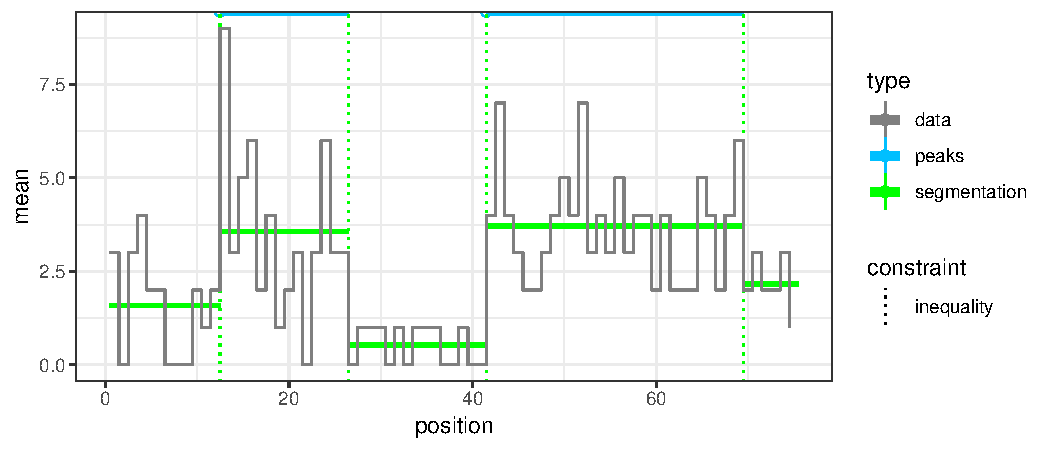
\includegraphics[width=\maxwidth]{figure/unnamed-chunk-5-1} 

}



\end{knitrout}

\section{Segment a data frame}

Another interface that can be used on a data.frame with $n$ rows and
exactly 4 columns (chrom, chromStart, chromEnd, count) is
\verb|PeakSegFPOP_df|. For each row $i\in\{1,\dots, n\}$, let
$z_i\in\mathbb Z_+$ be the non-negative count data (count column), and
let $w_i>0$ be the weight (equal to the number of bases,
chromEnd-chromStart). The optimization problem we solve is the same as
before. Note that this function does not perform run-length encoding
for you:

\begin{knitrout}
\definecolor{shadecolor}{rgb}{0.969, 0.969, 0.969}\color{fgcolor}\begin{kframe}
\begin{alltt}
\hlstd{(fit}\hlopt{$}\hlstd{df} \hlkwb{<-} \hlstd{PeakSegDisk}\hlopt{::}\hlkwd{PeakSegFPOP_df}\hlstd{(count.df,} \hlnum{10.5}\hlstd{))}
\end{alltt}
\begin{verbatim}
#> $segments
#>         chrom chromStart chromEnd     status     mean
#> 1: chrUnknown         69       75 background 2.166670
#> 2: chrUnknown         41       69       peak 3.714290
#> 3: chrUnknown         26       41 background 0.533333
#> 4: chrUnknown         12       26       peak 3.571430
#> 5: chrUnknown          0       12 background 1.583330
#> 
#> $loss
#>    penalty segments peaks bases bedGraph.lines mean.pen.cost total.loss
#> 1:    10.5        5     2    75             75    0.01507491  -19.86938
#>    equality.constraints mean.intervals max.intervals megabytes seconds
#> 1:                    0       4.633333             8 0.0344162   0.004
#> 
#> $data
#>          chrom chromStart chromEnd count
#>  1: chrUnknown          0        1     3
#>  2: chrUnknown          1        2     0
#>  3: chrUnknown          2        3     3
#>  4: chrUnknown          3        4     4
#>  5: chrUnknown          4        5     2
#>  6: chrUnknown          5        6     2
#>  7: chrUnknown          6        7     0
#>  8: chrUnknown          7        8     0
#>  9: chrUnknown          8        9     0
#> 10: chrUnknown          9       10     2
#> 11: chrUnknown         10       11     1
#> 12: chrUnknown         11       12     2
#> 13: chrUnknown         12       13     9
#> 14: chrUnknown         13       14     3
#> 15: chrUnknown         14       15     5
#> 16: chrUnknown         15       16     6
#> 17: chrUnknown         16       17     2
#> 18: chrUnknown         17       18     4
#> 19: chrUnknown         18       19     1
#> 20: chrUnknown         19       20     2
#> 21: chrUnknown         20       21     3
#> 22: chrUnknown         21       22     0
#> 23: chrUnknown         22       23     3
#> 24: chrUnknown         23       24     6
#> 25: chrUnknown         24       25     3
#> 26: chrUnknown         25       26     3
#> 27: chrUnknown         26       27     0
#> 28: chrUnknown         27       28     1
#> 29: chrUnknown         28       29     1
#> 30: chrUnknown         29       30     1
#> 31: chrUnknown         30       31     0
#> 32: chrUnknown         31       32     1
#> 33: chrUnknown         32       33     0
#> 34: chrUnknown         33       34     1
#> 35: chrUnknown         34       35     1
#> 36: chrUnknown         35       36     1
#> 37: chrUnknown         36       37     0
#> 38: chrUnknown         37       38     0
#> 39: chrUnknown         38       39     1
#> 40: chrUnknown         39       40     0
#> 41: chrUnknown         40       41     0
#> 42: chrUnknown         41       42     4
#> 43: chrUnknown         42       43     7
#> 44: chrUnknown         43       44     4
#> 45: chrUnknown         44       45     3
#> 46: chrUnknown         45       46     2
#> 47: chrUnknown         46       47     2
#> 48: chrUnknown         47       48     3
#> 49: chrUnknown         48       49     4
#> 50: chrUnknown         49       50     5
#> 51: chrUnknown         50       51     4
#> 52: chrUnknown         51       52     7
#> 53: chrUnknown         52       53     3
#> 54: chrUnknown         53       54     4
#> 55: chrUnknown         54       55     3
#> 56: chrUnknown         55       56     5
#> 57: chrUnknown         56       57     3
#> 58: chrUnknown         57       58     4
#> 59: chrUnknown         58       59     4
#> 60: chrUnknown         59       60     2
#> 61: chrUnknown         60       61     4
#> 62: chrUnknown         61       62     2
#> 63: chrUnknown         62       63     2
#> 64: chrUnknown         63       64     2
#> 65: chrUnknown         64       65     5
#> 66: chrUnknown         65       66     4
#> 67: chrUnknown         66       67     2
#> 68: chrUnknown         67       68     4
#> 69: chrUnknown         68       69     6
#> 70: chrUnknown         69       70     2
#> 71: chrUnknown         70       71     3
#> 72: chrUnknown         71       72     2
#> 73: chrUnknown         72       73     2
#> 74: chrUnknown         73       74     3
#> 75: chrUnknown         74       75     1
#>          chrom chromStart chromEnd count
#> 
#> attr(,"class")
#> [1] "PeakSegFPOP_df"  "PeakSegFPOP_dir" "list"
\end{verbatim}
\end{kframe}
\end{knitrout}

Note how \verb|bedGraph.lines| is now the same size as \verb|bases|,
75. The time/storage complexity is
log-linear in the number of \verb|bedGraph.lines|, so it is more efficient
to use the run-length encoding. This can be easily done in R:

\begin{knitrout}
\definecolor{shadecolor}{rgb}{0.969, 0.969, 0.969}\color{fgcolor}\begin{kframe}
\begin{alltt}
\hlstd{z.rle.vec} \hlkwb{<-} \hlkwd{rle}\hlstd{(z.rep.vec)}
\hlstd{chromEnd} \hlkwb{<-} \hlkwd{cumsum}\hlstd{(z.rle.vec}\hlopt{$}\hlstd{lengths)}
\hlstd{rle.df} \hlkwb{<-} \hlkwd{data.frame}\hlstd{(}
  \hlkwc{chrom}\hlstd{=}\hlstr{"chrUnknown"}\hlstd{,}
  \hlkwc{chromStart}\hlstd{=}\hlkwd{c}\hlstd{(}\hlnum{0L}\hlstd{, chromEnd[}\hlopt{-}\hlkwd{length}\hlstd{(chromEnd)]),}
  \hlstd{chromEnd,}
  \hlkwc{count}\hlstd{=z.rle.vec}\hlopt{$}\hlstd{values)}
\hlstd{gg.rle} \hlkwb{<-} \hlkwd{ggplot}\hlstd{()}\hlopt{+}
  \hlkwd{geom_segment}\hlstd{(}\hlkwd{aes}\hlstd{(}
    \hlstd{chromStart}\hlopt{+}\hlnum{0.5}\hlstd{, count,} \hlkwc{xend}\hlstd{=chromEnd}\hlopt{+}\hlnum{0.5}\hlstd{,} \hlkwc{yend}\hlstd{=count),}
    \hlkwc{data}\hlstd{=rle.df)}\hlopt{+}
  \hlkwd{geom_point}\hlstd{(}\hlkwd{aes}\hlstd{(}
    \hlstd{chromEnd, count),}
    \hlkwc{shape}\hlstd{=}\hlnum{1}\hlstd{,}
    \hlkwc{data}\hlstd{=rle.df)}\hlopt{+}
  \hlkwd{geom_vline}\hlstd{(}\hlkwd{aes}\hlstd{(}
    \hlkwc{xintercept}\hlstd{=changepoint,} \hlkwc{color}\hlstd{=model),}
    \hlkwc{data}\hlstd{=}\hlkwd{data.frame}\hlstd{(change.df,} \hlkwc{model}\hlstd{=}\hlstr{"simulation"}\hlstd{))}\hlopt{+}
  \hlkwd{scale_color_manual}\hlstd{(}
    \hlkwc{values}\hlstd{=}\hlkwd{c}\hlstd{(}
      \hlkwc{simulation}\hlstd{=}\hlstr{"black"}\hlstd{,}
      \hlkwc{fitted}\hlstd{=}\hlstr{"green"}\hlstd{))}\hlopt{+}
  \hlkwd{xlab}\hlstd{(}\hlstr{"position"}\hlstd{)}
\hlstd{gg.rle}
\end{alltt}
\end{kframe}

{\centering 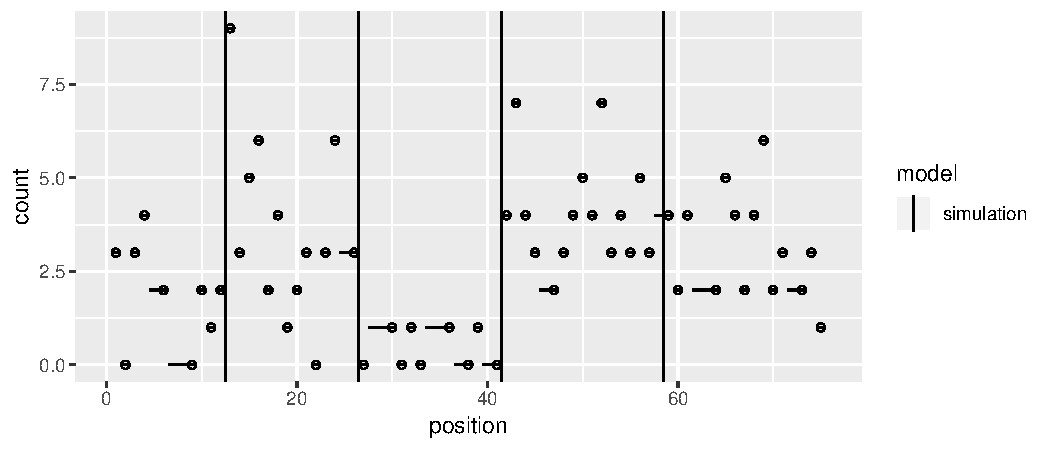
\includegraphics[width=\maxwidth]{figure/unnamed-chunk-7-1} 

}



\end{knitrout}

The plot above shows the run-length encoded data, with a \verb|geom_point|
for the last position in each run, and a \verb|geom_segment| extending left
to the first position. These data can be segmented as above:

\begin{knitrout}
\definecolor{shadecolor}{rgb}{0.969, 0.969, 0.969}\color{fgcolor}\begin{kframe}
\begin{alltt}
\hlstd{(fit}\hlopt{$}\hlstd{rle} \hlkwb{<-} \hlstd{PeakSegDisk}\hlopt{::}\hlkwd{PeakSegFPOP_df}\hlstd{(rle.df,} \hlnum{10.5}\hlstd{))}
\end{alltt}
\begin{verbatim}
#> $segments
#>         chrom chromStart chromEnd     status     mean
#> 1: chrUnknown         69       75 background 2.166670
#> 2: chrUnknown         41       69       peak 3.714290
#> 3: chrUnknown         26       41 background 0.533333
#> 4: chrUnknown         12       26       peak 3.571430
#> 5: chrUnknown          0       12 background 1.583330
#> 
#> $loss
#>    penalty segments peaks bases bedGraph.lines mean.pen.cost total.loss
#> 1:    10.5        5     2    75             60    0.01507491  -19.86938
#>    equality.constraints mean.intervals max.intervals  megabytes seconds
#> 1:                    0            4.6             8 0.02745438   0.003
#> 
#> $data
#>          chrom chromStart chromEnd count
#>  1: chrUnknown          0        1     3
#>  2: chrUnknown          1        2     0
#>  3: chrUnknown          2        3     3
#>  4: chrUnknown          3        4     4
#>  5: chrUnknown          4        6     2
#>  6: chrUnknown          6        9     0
#>  7: chrUnknown          9       10     2
#>  8: chrUnknown         10       11     1
#>  9: chrUnknown         11       12     2
#> 10: chrUnknown         12       13     9
#> 11: chrUnknown         13       14     3
#> 12: chrUnknown         14       15     5
#> 13: chrUnknown         15       16     6
#> 14: chrUnknown         16       17     2
#> 15: chrUnknown         17       18     4
#> 16: chrUnknown         18       19     1
#> 17: chrUnknown         19       20     2
#> 18: chrUnknown         20       21     3
#> 19: chrUnknown         21       22     0
#> 20: chrUnknown         22       23     3
#> 21: chrUnknown         23       24     6
#> 22: chrUnknown         24       26     3
#> 23: chrUnknown         26       27     0
#> 24: chrUnknown         27       30     1
#> 25: chrUnknown         30       31     0
#> 26: chrUnknown         31       32     1
#> 27: chrUnknown         32       33     0
#> 28: chrUnknown         33       36     1
#> 29: chrUnknown         36       38     0
#> 30: chrUnknown         38       39     1
#> 31: chrUnknown         39       41     0
#> 32: chrUnknown         41       42     4
#> 33: chrUnknown         42       43     7
#> 34: chrUnknown         43       44     4
#> 35: chrUnknown         44       45     3
#> 36: chrUnknown         45       47     2
#> 37: chrUnknown         47       48     3
#> 38: chrUnknown         48       49     4
#> 39: chrUnknown         49       50     5
#> 40: chrUnknown         50       51     4
#> 41: chrUnknown         51       52     7
#> 42: chrUnknown         52       53     3
#> 43: chrUnknown         53       54     4
#> 44: chrUnknown         54       55     3
#> 45: chrUnknown         55       56     5
#> 46: chrUnknown         56       57     3
#> 47: chrUnknown         57       59     4
#> 48: chrUnknown         59       60     2
#> 49: chrUnknown         60       61     4
#> 50: chrUnknown         61       64     2
#> 51: chrUnknown         64       65     5
#> 52: chrUnknown         65       66     4
#> 53: chrUnknown         66       67     2
#> 54: chrUnknown         67       68     4
#> 55: chrUnknown         68       69     6
#> 56: chrUnknown         69       70     2
#> 57: chrUnknown         70       71     3
#> 58: chrUnknown         71       73     2
#> 59: chrUnknown         73       74     3
#> 60: chrUnknown         74       75     1
#>          chrom chromStart chromEnd count
#> 
#> attr(,"class")
#> [1] "PeakSegFPOP_df"  "PeakSegFPOP_dir" "list"
\end{verbatim}
\begin{alltt}
\hlstd{gg.rle}\hlopt{+}
  \hlkwd{geom_segment}\hlstd{(}\hlkwd{aes}\hlstd{(}
    \hlstd{chromStart}\hlopt{+}\hlnum{0.5}\hlstd{, mean,} \hlkwc{xend}\hlstd{=chromEnd}\hlopt{+}\hlnum{0.5}\hlstd{,} \hlkwc{yend}\hlstd{=mean,} \hlkwc{color}\hlstd{=model),}
    \hlkwc{data}\hlstd{=}\hlkwd{data.frame}\hlstd{(fit}\hlopt{$}\hlstd{rle}\hlopt{$}\hlstd{segments,} \hlkwc{model}\hlstd{=}\hlstr{"fitted"}\hlstd{))}
\end{alltt}
\end{kframe}

{\centering 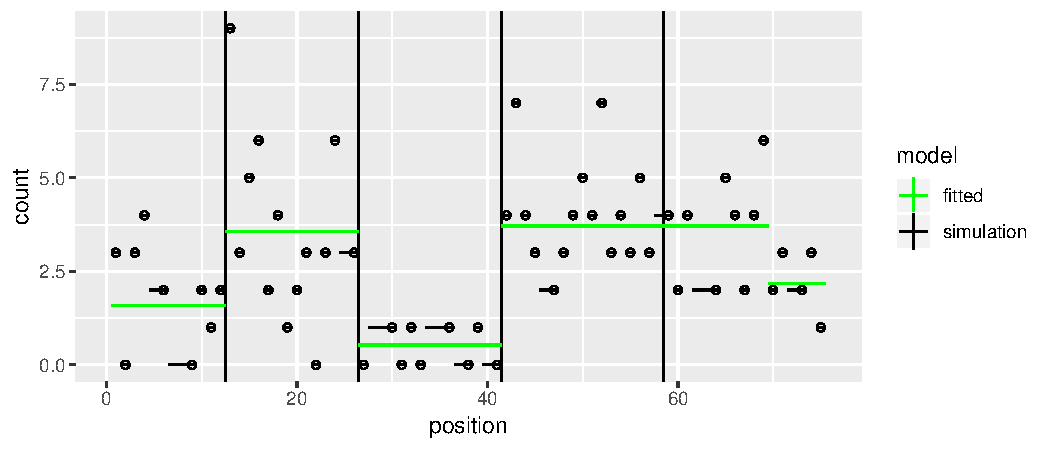
\includegraphics[width=\maxwidth]{figure/unnamed-chunk-8-1} 

}



\end{knitrout}

\section{Write the file yourself}

The interfaces discussed in the previous sections are perhaps the most
intuitive for useRs, but they are also the least efficient, so they
are not recommended for large data. 

In this section we introduce the most efficient way of using PeakSegDisk, which involves:

\begin{itemize}
\item creating a ``problem'' directory for each segmentation problem
  (sample and genome subset),
\item saving the data to \verb|coverage.bedGraph| in that directory,
\item and then running \verb|PeakSegFPOP_dir|.
\end{itemize}

The reason why this method is recommended for large data is because
\verb|PeakSegFPOP_dir| saves its results to the ``problem'' directory. So
if a certain result has already been computed, these result files are
used as a cache, and are read instead of doing computations, which
saves a lot of time. 
The file system is used as the interface in
order to support very large data sets with very little memory usage.

To use \verb|PeakSegFPOP_dir| the data should be saved to a
chrXX-start-end/coverage.bedGraph file, where the problem directory
``chrXX-start-end'' should be named using a genome postion string:

\begin{itemize}
\item chrXX is the chromosome (which is irrelevant to the algorithm),
\item start is the 0-based first position of the region to segment (the smallest possible value is 0),
\item end is the 1-based end position (the smallest possible value is 1).
\end{itemize}

\begin{knitrout}
\definecolor{shadecolor}{rgb}{0.969, 0.969, 0.969}\color{fgcolor}\begin{kframe}
\begin{alltt}
\hlstd{data.dir} \hlkwb{<-} \hlkwd{file.path}\hlstd{(}
  \hlkwd{tempfile}\hlstd{(),}
  \hlkwd{with}\hlstd{(rle.df,} \hlkwd{sprintf}\hlstd{(}
    \hlstr{"%s-%d-%d"}\hlstd{, chrom[}\hlnum{1}\hlstd{],} \hlkwd{min}\hlstd{(chromStart),} \hlkwd{max}\hlstd{(chromEnd))))}
\hlkwd{dir.create}\hlstd{(data.dir,} \hlkwc{showWarnings}\hlstd{=}\hlnum{FALSE}\hlstd{,} \hlkwc{recursive}\hlstd{=}\hlnum{TRUE}\hlstd{)}
\hlstd{coverage.bedGraph} \hlkwb{<-} \hlkwd{file.path}\hlstd{(data.dir,} \hlstr{"coverage.bedGraph"}\hlstd{)}
\hlkwd{write.table}\hlstd{(}
  \hlstd{rle.df, coverage.bedGraph,}
  \hlkwc{sep}\hlstd{=}\hlstr{"\textbackslash{}t"}\hlstd{,} \hlkwc{row.names}\hlstd{=}\hlnum{FALSE}\hlstd{,} \hlkwc{col.names}\hlstd{=}\hlnum{FALSE}\hlstd{)}
\end{alltt}
\end{kframe}
\end{knitrout}

The next step is to run the main solver, 

\begin{knitrout}
\definecolor{shadecolor}{rgb}{0.969, 0.969, 0.969}\color{fgcolor}\begin{kframe}
\begin{alltt}
\hlstd{(fit}\hlopt{$}\hlstd{dir} \hlkwb{<-} \hlstd{PeakSegDisk}\hlopt{::}\hlkwd{PeakSegFPOP_dir}\hlstd{(data.dir,} \hlnum{10.5}\hlstd{))}
\end{alltt}
\begin{verbatim}
#> $segments
#>         chrom chromStart chromEnd     status     mean
#> 1: chrUnknown         69       75 background 2.166670
#> 2: chrUnknown         41       69       peak 3.714290
#> 3: chrUnknown         26       41 background 0.533333
#> 4: chrUnknown         12       26       peak 3.571430
#> 5: chrUnknown          0       12 background 1.583330
#> 
#> $loss
#>    penalty segments peaks bases bedGraph.lines mean.pen.cost total.loss
#> 1:    10.5        5     2    75             60    0.01507491  -19.86938
#>    equality.constraints mean.intervals max.intervals  megabytes seconds
#> 1:                    0            4.6             8 0.02745438   0.003
#> 
#> attr(,"class")
#> [1] "PeakSegFPOP_dir" "list"
\end{verbatim}
\end{kframe}
\end{knitrout}

The
underlying C++ code
creates penalty-specific files such as

\verb|chrXX-start-end/coverage.bedGraph_penalty=0.1_loss.tsv| which
are used to store/cache the results.  If the files already exist (and
are consistent) then \verb|PeakSegFPOP_dir| just reads them; otherwise
it runs the dynamic programming C++ code in order to create those
files, which are then read into R.

\section{Computing the model with a given number of peaks}

The \verb|sequentialSearch_dir| function can be used to compute the
optimal model with a certain number of peaks:

\begin{knitrout}
\definecolor{shadecolor}{rgb}{0.969, 0.969, 0.969}\color{fgcolor}\begin{kframe}
\begin{alltt}
\hlkwa{if}\hlstd{(}\hlkwd{interactive}\hlstd{()} \hlopt{&&} \hlkwd{requireNamespace}\hlstd{(}\hlstr{"future"}\hlstd{))future}\hlopt{::}\hlkwd{plan}\hlstd{(}\hlstr{"multiprocess"}\hlstd{)}
\hlstd{(fit}\hlopt{$}\hlstd{search} \hlkwb{<-} \hlstd{PeakSegDisk}\hlopt{::}\hlkwd{sequentialSearch_dir}\hlstd{(data.dir,} \hlnum{2L}\hlstd{,} \hlkwc{verbose}\hlstd{=}\hlnum{1}\hlstd{))}
\end{alltt}


{\ttfamily\noindent\itshape\color{messagecolor}{\#> Loading required namespace: future.apply}}\begin{verbatim}
#> Next = 0, Inf 
#> Next = 2.20991803112367 
#> Next = 7.11950550040458
#> $segments
#>         chrom chromStart chromEnd     status     mean
#> 1: chrUnknown         69       75 background 2.166670
#> 2: chrUnknown         41       69       peak 3.714290
#> 3: chrUnknown         26       41 background 0.533333
#> 4: chrUnknown         12       26       peak 3.571430
#> 5: chrUnknown          0       12 background 1.583330
#> 
#> $loss
#>     penalty segments peaks bases bedGraph.lines mean.pen.cost total.loss
#> 1: 7.119506        5     2    75             60   -0.07507161  -19.86938
#>    equality.constraints mean.intervals max.intervals  megabytes seconds
#> 1:                    0       4.558333             9 0.02735901   0.003
#>    iteration under over
#> 1:         3     0    6
#> 
#> $others
#>     penalty segments peaks bases bedGraph.lines mean.pen.cost total.loss
#> 1: 0.000000       53    26    75             60   -0.63772877 -47.829658
#> 2:      Inf        1     0    75             60    0.12837615   9.628211
#> 3: 2.209918       13     6    75             60   -0.26439085 -33.088822
#> 4: 7.119506        5     2    75             60   -0.07507161 -19.869382
#>    equality.constraints mean.intervals max.intervals  megabytes seconds
#> 1:                    5       2.550000             4 0.02276230   0.003
#> 2:                    0       0.000000             0 0.00000000   0.001
#> 3:                    0       4.708333             9 0.02770233   0.003
#> 4:                    0       4.558333             9 0.02735901   0.003
#>    iteration under over
#> 1:         1    NA   NA
#> 2:         1    NA   NA
#> 3:         2     0   26
#> 4:         3     0    6
#> 
#> attr(,"class")
#> [1] "PeakSegFPOP_dir" "list"
\end{verbatim}
\end{kframe}
\end{knitrout}

The algorithm must evaluate several penalty values to compute the
optimal model with a certain number of peaks. The \verb|others| component of
the model list above shows that

\begin{itemize}
\item the search starts with penalty values 0 and Inf, which result in models
  with 26 and 0 peaks, respectively.
\item the next penalty evaluated is 2.21, 
  which results in 6 peaks.
\item the final penalty evaluated is 7.12, 
  which results in 2 peaks.
\end{itemize}
  
At each step (except the first) the new penalties are computed based
on the loss values found in the previous step. 
If present with a registered parallel future plan, 
the \verb|future.apply| package is used to run the first step 
(penalties $0,\infty$) in parallel.

Note how the number of peaks and \verb|total.loss| of this model is
the same as the other models computed above,

\begin{knitrout}
\definecolor{shadecolor}{rgb}{0.969, 0.969, 0.969}\color{fgcolor}\begin{kframe}
\begin{alltt}
\hlstd{lossDF} \hlkwb{<-} \hlkwa{function}\hlstd{(}\hlkwc{L}\hlstd{)}\hlkwd{data.frame}\hlstd{(L}\hlopt{$}\hlstd{loss)[,} \hlkwd{names}\hlstd{(fit}\hlopt{$}\hlstd{dir}\hlopt{$}\hlstd{loss)]}
\hlkwd{do.call}\hlstd{(rbind,} \hlkwd{lapply}\hlstd{(fit, lossDF))}
\end{alltt}
\begin{verbatim}
#>          penalty segments peaks bases bedGraph.lines mean.pen.cost
#> vec    10.500000        5     2    75             60    0.01507491
#> df     10.500000        5     2    75             75    0.01507491
#> rle    10.500000        5     2    75             60    0.01507491
#> dir    10.500000        5     2    75             60    0.01507491
#> search  7.119506        5     2    75             60   -0.07507161
#>        total.loss equality.constraints mean.intervals max.intervals
#> vec     -19.86938                    0       4.600000             8
#> df      -19.86938                    0       4.633333             8
#> rle     -19.86938                    0       4.600000             8
#> dir     -19.86938                    0       4.600000             8
#> search  -19.86938                    0       4.558333             9
#>         megabytes seconds
#> vec    0.02745438   0.011
#> df     0.03441620   0.004
#> rle    0.02745438   0.003
#> dir    0.02745438   0.003
#> search 0.02735901   0.003
\end{verbatim}
\end{kframe}
\end{knitrout}

Finally we demonstrate how the filesystem caching is especially useful
for the sequential search. In the code below we ask the sequential
search algorithm to compute the optimal model with four peaks:

\begin{knitrout}
\definecolor{shadecolor}{rgb}{0.969, 0.969, 0.969}\color{fgcolor}\begin{kframe}
\begin{alltt}
\hlstd{four.peaks} \hlkwb{<-} \hlstd{PeakSegDisk}\hlopt{::}\hlkwd{sequentialSearch_dir}\hlstd{(data.dir,} \hlnum{4L}\hlstd{)}
\end{alltt}


{\ttfamily\noindent\itshape\color{messagecolor}{\#> Loading required namespace: future.apply}}\begin{alltt}
\hlstd{four.peaks}\hlopt{$}\hlstd{others[,} \hlkwd{.}\hlstd{(iteration, penalty, peaks)]}
\end{alltt}
\begin{verbatim}
#>    iteration  penalty peaks
#> 1:         1 0.000000    26
#> 2:         1      Inf     0
#> 3:         2 2.209918     6
#> 4:         3 7.119506     2
#> 5:         4 3.304860     3
#> 6:         5 2.830674     5
#> 7:         6 3.107790     4
\end{verbatim}
\end{kframe}
\end{knitrout}

Looking at the output above, we see that the first three iterations of
the sequential search require computing models with 26, 0, 6, 2
peaks. Since all of these have been previously computed (and saved to
disk), the dynamic programming algorithm does not need to be re-run,
and instead the model results are simply read from the files. After
that the dynamic programming is run for the subsequent iterations
4-6. In this particular example the savings in computation time is not
extraordinary, but in real genomic data, this can result in
substantial speed-ups.

\end{document}
